\documentclass[utf8,draft]{frontiersFPHY} % for Physics and Applied Maths
\usepackage{graphicx}
\usepackage{amssymb}
\usepackage{siunitx}
\usepackage{amsmath}
\usepackage{soul}
\usepackage{physics}
\usepackage{bm}

\usepackage{url,hyperref,microtype,subcaption}
\usepackage[onehalfspacing]{setspace}
\usepackage{cleveref}
% \usepackage[font={bold,it}]{caption}

\graphipath{{../figures/}}

% Define better ref abbreviations
\usepackage[displaymath]{lineno}

% Define some convenience commands
\renewcommand{\d}{\mathrm{d}}
\renewcommand{\k}{\mathrm{K}}
\newcommand{\ca}{\mathrm{Ca}}
\newcommand{\na}{\mathrm{Na}}
\newcommand{\leak}{\mathrm{L}}
\newcommand{\dstar}{d^\star}
\newcommand{\gstar}{g^\star}
\newcommand{\gbar}{\bar g}
\newcommand{\delt}{\Delta t}
\newcommand{\taus}{\tau_s}
\newcommand{\dn}{\delta_n}
\newcommand{\taud}{\tau_d}


\linenumbers


\def\keyFont{\fontsize{8}{11}\helveticabold }
\def\firstAuthorLast{Olenik {et~al.}} %use et al only if is more than 1 author
\def\Authors{Mark Olenik\,$^{1,*}$, and Conor Houghton\,$^{2}$}
% Affiliations should be keyed to the author's name with superscript numbers and be listed as follows: Laboratory, Institute, Department, Organization, City, State abbreviation (USA, Canada, Australia), and Country (without detailed address information such as city zip codes or street names).
% If one of the authors has a change of address, list the new address below the correspondence details using a superscript symbol and use the same symbol to indicate the author in the author list.
\def\Address{$^{1}$School of Biological Sciences, Faculty of Life Sciences, University of Bristol, Bristol, United Kingdom \\
$^{2}$School of Computer Science, Electrical and Electronic Engineering, and Engineering Mathematics, Faculty of Engineering, University of Bristol, Bristol, United Kingdom}
% The Corresponding Author should be marked with an asterisk
% Provide the exact contact address (this time including street name and city zip code) and email of the corresponding author
\def\corrAuthor{Mark Olenik}

\def\corrEmail{m.olenik@bristol.ac.uk}


\begin{document}

\onecolumn
\firstpage{1}


\title[Scalar Poincaré map for bursting]{A scalar Poincaré map for anti-phase bursting in coupled inhibitory neurons with synaptic depression.}


\author[\firstAuthorLast ]{\Authors} %This field will be automatically populated
\address{} %This field will be automatically populated
\correspondance{} %This field will be automatically populated

\extraAuth{}% If there are more than 1 corresponding author, comment this line and uncomment the next one.
%\extraAuth{corresponding Author2 \\ Laboratory X2, Institute X2, Department X2, Organization X2, Street X2, City X2 , State XX2 (only USA, Canada and Australia), Zip Code2, X2 Country X2, email2@uni2.edu}


\maketitle

\begin{abstract}
\section{}
Short-term synaptic plasticity is found in many areas of the central
nervous system.  In the inhibitory half-centre central pattern
generators involved in locomotion, synaptic depression is believed to
act as a burst termination mechanism, allowing networks to generate
anti-phase bursting patterns of varying periods.  To better understand
burst generation in these central patter generators, we study a
minimal network of two neurons coupled through depressing synapses.
Depending on the strength of the synaptic conductance between the two
neurons, this network can produce symmetric $n-n$ anti-phase bursts,
where neurons fire $n$ spikes in alternation, with the period of such
solutions increasing with the strength of the synaptic conductance.
Relying on the timescale disparity in the model, we reduce the
eight-dimensional network equations to a fully-explicit scalar
Poincaré burst map.  This map tracks the state of synaptic depression
from one burst to the next and captures the complex bursting dynamics
of the network.  Fixed points of this map are associated with stable
burst solutions of the full network model, and are created through
fold bifurcations of maps.  We derive conditions that describe
period-increment bifurcations between stable $n-n$ and $(n+1)-(n+1)$
bursts, producing a full bifurcation diagram of the burst cycle
period.  Predictions of the Poincaré map fit excellently with
numerical simulations of the full network model and allow the study of
parameter sensitivity for rhythm generation.


\tiny
 \keyFont{ \section{Keywords:} Synaptic depression, Poincaré map, Dynamical system, Neuronal bursting, Central pattern generator}

\end{abstract}



\section{Introduction}
% DEPRESSION
Short-term synaptic plasticity may have a role in burst activity in
central pattern generators (CPGs).  Short-term synaptic depression is
commonly found in neuronal networks involved in the generation of
rhythmic movements, such as in the pyloric CPG of the spiny
lobster~\citep{manor1997, rabbah2007}, or in the lumbosacral cord of
the chick embryo~\citep{donovan1998}.  Synaptic depression modulates
the strength of synapses in response to changes to the presynaptic
firing frequency.  At a high neuronal firing frequency, depression
weakens the strength of synapses and therefore reduces the magnitude
of the postsynaptic response.  At low firing frequency, it allows
sufficient time for the synapse to recover from depression between
spikes, leading to a stronger postsynaptic response.  In reciprocal
networks, synaptic depression has been shown to act as a ``switch'',
giving rise to a wide range of network dynamics such as synchronous
and multi-stable rhythms, as well as fine tuning the frequency of
network oscillations~\citep{nadim2000, nadim1999, bose2011}.

% Brown
~\citet{brown1911} pioneered the idea that synaptic depression acts as
a burst termination mechanism in reciprocally inhibitory CPGs involved
in rhythm generation of locomotion. When one side is firing during a
burst the other, antagonistic side, is prevented from firing by
synaptic inhibition. However, the weakening of inhibition as a result
of synaptic depression eventually releases the antagonistic side so
that it starts firing, terminating the burst on the side that had
originally been firing.  This rhythmogenesis hypothesis has been
considered one of a handful of standard mechanisms for generating
locomotion rhythms in
vertebrates~\citep{reiss1962,perkel1974,friesen1994}. It has been
proposed as an explaination of the antiphase burst rhythm in
struggling in \textit{Xenopus} tadpoles~\citep{li2007}.

~\citet{bose2011} investigated burst generation in a generic
half-centre CPG that consists of two identical, tonically active
Morris-Lecar~\citep{morris1981} neurons coupled through inhibitory
depressing synapses.  Numerical simulations showed that when the
reciprocal synaptic conductance between the two neurons is varied, the
network produces symmetric $n-n$ anti-phase bursts, with stronger
synaptic coupling leading to longer bursts.  They used methods from
geometric singular perturbation theory to separate the timescales of
the fast membrane, and the slow synaptic dynamics of the network to
derive one-dimensional conditions necessary for the existence of
stable $n-n$ solutions (for $n\leq 2$). According to these conditions
the type of firing pattern largely depends on the slow depression
dynamics of the synapses between the two neurons, and can therefore be
predicted by knowing the strengths of the synaptic conductances of the
two synapses.
Thus, the scalar conditions derived in~\citet{bose2011} provide a
method to numerically identify the type of stable $n-n$ pattern for
any given value of the coupling strength.  However, they do not
predict the exact period of such solutions.
Furthermore, while they provide good arguments for the validity of
their reduction assumptions and the resulting scalar conditions, they
do not verify them numerically.

Here we extend the previous analysis by providing a Poincaré map of
the slow depression dynamics.  This allows us not only to predict the
types of stable $n-n$ solutions the full network can produce, (for any
$n$), but also to study how varying the coupling strength affects the
period of such solutions.  To do this, we build on, and numerically
test, the assumptions on the fast-slow timescale disparity made
in~\cite{bose2011}.  We reduce the two-cell model to a scalar
Poincaré map that tracks the evolution of the depression from the
beginning of one burst to the beginning of the next burst.  Stable
fixed points of our map are associated with stable $n-n$ burst
solutions.  Our map construction is motivated by the burst length map
of a T-type calcium current, utilised by~\citet{matveev2007}, which
approximates the anti-phase bursting dynamics of a network of two
coupled Morris-Lecar neurons.  In contrast to our model, the network
described in the~\cite{matveev2007} paper does not contain short-term synaptic
depression, and burst termination is instead accomplished through the
dynamics of a slow T-type calcium current.

% MAIN RESULTS AND CONCLUSIONS
The Poincaré map derived here replicates the results from numerical
simulations of the full two-cell ODE system: Given the strength of
maximum conductance between the two neurons, fixed points of our map
predict the type and period of $n-n$ patterns, the switch between
burst solutions of different periods, as well as the occurrence of
co-existent solutions.  In addition to proving the existence and
stability of fixed points, our map shows that fixed points are created
via a fold bifurcation of maps.  We also derive algebraic conditions
that predict the period increment bifurcations that allow the switch
between $n-n$ and $(n+1)-(n+1)$ solutions.  Because our map is fully
explicit, it lays the framework for studying the effects of other
model parameter on network dynamics without the need to run expensive
numerical integrations of the ODEs.

% PAPER STRUCTURE.
This paper is organised as follows.  First, we introduce the network
of two neurons, and describe the properties of single cell and synapse
dynamics.  We use numerical simulations of the network to provide an
intuition for the range of possible burst dynamics the system can
produce.  Next, we state and justify the simplifying assumptions that
are necessary for the map construction.  Finally, we analytically
derive the first return map of the depression variable as well as the
conditions that are required for stable solutions to bifurcate between
$n-n$ and $(n+1)-(n+1)$ solutions.  We end this work with a
discussion.

\section{Materials and Methods}
We consider a pair of identical Morris-Lecar neurons~\citep{morris1981}, with parameters adapted from~\cite{bose2011}.
The Morris-Lecar model is a set of two first-order differential equations that describe the membrane dynamics of a spiking neuron.
The depolarisation is modelled by an instantaneous calcium current, and the hyperpolarisation by a slow potassium current and a leak current.
The membrane potential $v_{i}$ and potassium activation $w_{i}$ of neuron $i$ ($i, j=1,2$) is described by:
\begin{align}
    ~\label{eq:cell-modelA}
     \dot v_{i}&= f(v_{i}, w_{i}) -\gbar s_j(v_i-v_{s}),\\
    ~\label{eq:cell-modelB}
     \dot w_{i} &=h(v_i,w_i).
   \end{align}
Here $v_{s}$ is the inhibitory reversal potential, and $\gbar$ and $s_{j}$ are the maximal synaptic conductance and the synaptic gating, respectively, constituting the total inhibitory conductance $\gbar s_{j}$ from neuron $j$ to neuron $i$.
Function $f(v_{i}, w_{i})$ describes the membrane currents of a single cell:
\begin{equation}
 ~\label{eq:memcur}
  f(v_{i}, w_{i}) = -g_{\ca}m_{\infty}(v_{i})(v_{i}-v_{\ca}) - g_{\k}w_{i}(v_{i}-v_{\k})-g_{\leak}(v_{i}-v_{\leak}) + I.
\end{equation}
The currents include a constant current $I$, and three ionic currents:
an instantaneous calcium current, a potassium current, and a leak current, with respective reversal potentials $v_{\ca}$, $v_{\k}$, and $v_{\leak}$, as well as maximum conductances $g_{\ca}$, $g_{\k}$, and $g_{\leak}$.
The function $h(v_{i}, w_{i})$ models the kinetics of the potassium gating variable $w_{i}$, and is given by
\begin{equation}
  h(v_{i}, w_{i})=\frac{w_{\infty}(v_{i})-w_{i}}{\tau_{w}}~\label{eq:h}.
\end{equation}
The steady-state activation functions $m_{\infty}$ and $w_{\infty}$ as well as the default model parameters are described in the \textbf{Supplementary Material S1}.

The dynamics of the synaptic interactions between the neurons are governed by a synaptic gating variable $s_{i}$ and a depression variable $d_{i}$:
\begin{linenomath}
  \begin{align}
    \dot s_{i} &= -s_{i}/\tau_{s}~\label{eq:dot-s},\\
    \dot d_{i} &= (1-d_{i})/\tau_{d}~\label{eq:dot-d}.
  \end{align}
\end{linenomath}
Variable $d_{i}$ describes a firing rate dependent depletion mechanism that governs the amount of depression acting on the synapse.
Our model is agnostic with respect to the exact mechanism of this depletion, be it pre- or post-synaptic.
In between spikes $s_{i}$ decays with time constant $\tau_{s}$, while $d_{i}$ recovers with time constant $\tau_{d}$.
Because synaptic depression occurs on a much slower timescale than synaptic inhibition, we assume $\tau_{d}\gg\tau_{s}$.
At spike time when the voltage $v_{i}$ crosses a synaptic threshold $v_{\theta}$, the synaptic variable $s_{i}$ is reset to the current value of $d_{i}$, and $d_{i}$ is scaled down by the depression strength parameter $\lambda$, where $0<\lambda<1$.
This results in the following discontinuous reset rule on spike time:
\begin{linenomath}
  \begin{align}
    s_{i} &\leftarrow d_{i}~\label{eq:s-reset},\\
    d_{i} &\leftarrow \lambda d_{i}~\label{eq:d-reset}.
  \end{align}
\end{linenomath}
The equations for the depression model were adapted from the~\citet{bose2001} model.
These equations are a mathematically tractable simplification of the established phenomenological depression model previously described by~\citet{tsodyks1997}.
The original equations in~\cite{bose2001} include an exponential decay of $d_{i}$ throughout the active phase of the action potential, that is $\dot d_{i}=-d_{i}/\tau_{\beta}$ for $v_{i}>v_{\theta}$.
To simplify the mathematical analysis we have reduced these dynamics to a single-reset event at spike time according to \cref{eq:d-reset}.
This simplification is natural given an approximately constant duration of the active phase of an action potential, and it will become evident from our results that this simplification does not qualitatively change the dynamics of the network compared to the original equations, where depression dynamics are described by an exponential decay.

When the cells are uncoupled ($\gbar=0$), the membrane dynamics are determined by the cubic $v$-nullcline $v_{\infty}(v_i)$ and the sigmoid $w$-nullcline $w_{\infty}(v_{i})$, satisfying $\dot v_{i}=0$ and $\dot w_{i}=0$, respectively.
The two curves intersect along the middle branch of $v_{\infty}$, creating an unstable fixed point $p_{f}=(v_{f},w_{f})$ with a surrounding stable limit cycle of period $T$ (\cref{fig:nullclines}A).
Trajectories along that limit cycle have the familiar shape of the action potential (\cref{fig:nullclines}B).
The trajectory of an action potential can be dissected into four phases: (1) a silent phase, (2) a jump up, (3) an active phase, and (4) a jump down~\citep[see e.g.][]{ermentrout2010}.
During the silent phase the trajectory evolves along the left branch ($v_{i}<v_{\theta}$) of the cubic $v$-nullcline.
Once the trajectory reaches the local minimum of $v_{\infty}$, it ``jumps up'' to the right branch ($v_{i}>v_{\theta}$), crossing the firing threshold $v_{\theta}$.
During the active phase the trajectory then evolves along the right branch of the cubic until it arrives at the local maximum, where it ``jumps down'' to the left branch commencing a new cycle.

The two-cell network model is numerically integrated using an adaptive step-size integrator for stiff differential equations implemented with XPPAUT~\citep{ermentrout2002} and controlled through the Python packages SciPy~\citep{scipy2020} and PyXPP~\citep{pyxpp}.
The following mathematical analysis is performed on the equations of a single cell.
Unless required for clarity, we will therefore omit the subscripts $i,j$ from here on.

\section{Results}
\subsection{Anti-phase burst solutions}
Short-term synaptic depression of inhibition in a half-centre oscillator acts as a \emph{burst termination} mechanism~\citep{brown1911} and is known to produce $n-n$ anti-phase burst solutions of varying period.
Such $n-n$ solutions consist of cells firing bursts of $n$ spikes in alternation.
\Cref{fig:depression-traces}A shows the timecourse of a typical $4-4$ burst.
While one cell is firing a burst it provides an inhibitory conductance to the other cell,  preventing it from firing.
Therefore, at any given moment one cell is spiking while the other is inhibited.
Consistent with~\citet{bose2011} we will refer to the currently firing cell as ``free'' and we will call the inhibited cell ``quiet''.
Additionally, we will distinguish between two phases of a $n-n$ solution:
We will refer to the burst duration of a cell as the ``free phase'', which is the time between the first spike and the last spike in a burst. And we will call the remaining duration of a cycle, when a cell is not spiking, the ``quiet phase''.

% TODO: Add mention of gstar. Once critical conductance is crossed, cell is released.
With each action potential of the free cell, short-term depression leads to a step-wise decrease of $d$, and consequently of $s$ (\cref{fig:depression-traces}B).
If $d$ depresses faster at spike time than it can recover in the inter-spike-intervals ($ISI$s), the total synaptic conductance $\gbar s$ will eventually become sufficiently small to allow for the quiet cell to be released and start firing, thus inhibiting the previously free cell.
While a cell is quiet its depression variable can recover.
Once the quiet cell becomes free again its synaptic inhibition will be sufficient to terminate the burst of the previously free cell and commence a new cycle.
As previously demonstrated by~\citet{bose2011}, in a two-cell reciprocally inhibitory network with synaptic depression the coupling strength $\gbar$ determines the type of $n-n$ solution.
Increasing $\gbar$ produces higher $n-n$ burst solutions with more spikes per burst and a longer cycle period.
\Cref{fig:burst-sols} shows numerically stable $n-n$ solutions for varying values of $\gbar$.
For small values of $\gbar$ the network produces anti-phase spiking $1-1$ solutions.
As $\gbar$ is increased the network generates solutions of increasing $n$, that is $2-2$, $3-3$, and $4-4$.
When $\gbar$ is sufficiently large (bottom of \cref{fig:burst-sols}), one of the cells continuously spikes at its uncoupled period $T$ while the other cell remains fully suppressed.
Depending on the initial conditions either of the two cells can become the suppressed cell, which is why the suppressed solution is numerically bistable.

Branches of numerically stable $n-n$ solutions and their associated limit cycle period for varying values of $\gbar$ are depicted in \cref{fig:bif-diagram}A (see  \textbf{Supplementary Material S2} for algorithm description).
Not only do higher $n-n$ solutions branches require stronger coupling $\gbar$, but also within $n-n$ branches the period increases with $\gbar$.
In line with~\citet{bose2011} we find small overlaps between solution branches indicating numerical bistability, for example such as between the $2-2$ and $3-3$ solution branches.
Branches of higher $n-n$ burst solutions occur on increasingly smaller intervals of $\gbar$, for instance is the $\gbar$ interval of the $5-5$ branch shorter than that of the $4-4$ branch and so on.
The interval between the $5-5$ branch and the suppressed solution (region between dotted lines in \cref{fig:bif-diagram}A) not only contains even higher numerically stable $n-n$ solutions, such as $11-11$ bursts, but also other non-symmetric $n-m$ solutions as well irregular, non-periodic solutions. However, the analysis in the following sections will only be concerned with the numerically stable and symmetric $n-n$ solutions.

\subsection{Mathematical analysis of two-cell network}
~\label{sec:assumptions}
% Summary of assumptions
The goal of the following mathematical analysis is to reduce the complexity of the eight-dimensional system to some easily tractable quantity.
As we will see later this quantity is the value of the depression variable $d$ of either of the two cells.
We will construct the solution of $d$ in a piecewise manner from one spike to the next, first during the free phase, and then during the quiet phase.
This construction will require two assumptions about the membrane and synaptic dynamics.
The first assumption states that during a burst the free cell fires at its uncoupled period $T$, which simplifies the construction of the solution of $d$.
The second assumption states that once the inhibitory conductance acting on the quiet cell drops below a critical threshold, the cell is immediately released and fires.
The second assumption is necessary to predict the release time of the quiet cell, which allows us to model the recovery of $d$ during the quiet phase.
In other words, the second assumption requires that the release of the quiet cell from inhibition depends only on the timecourse of the inhibition, and not on the membrane dynamics of the quiet cell.
Both assumptions can be observed in coupled relaxation-oscillator types of neurons such as the Morris-Lecar model we use, and will be numerically verified below.
Both assumptions were first explored in~\cite{bose2011} to derive algebraic conditions that guarantee the periodicity of the depression variable for different $n-n$ solutions.
However here we will use these assumptions to construct a Poincaré map of $d$, which will provide a geometric intuition for the dynamics of the full two-cell network and its dependence on model parameters.

% Assumption 1: Free phase
Our first assumption about the model states that the free cell fires at its uncoupled period $T$, that is, during the free phase of a burst we have $ISI=T$.
Solution profiles in \cref{fig:burst-sols} suggest that the $ISI$s are indeed approximately constant.
We can further numerically confirm this observation by capturing the $ISI$s of the stable solutions from the bifurcation diagram in \cref{fig:bif-diagram}A.
In addition to $ISI$s, \Cref{fig:bif-diagram}B also shows inter-\textit{burst} intervals ($IBI$s), which correspond to the time interval between the last spike of the burst and the full cycle period, and which lie in the quiet phase of the burst.
$IBI$s lie on multiple branches, each branch associated with a stable $n-n$ solution, and are monotonically increasing with $\gbar$.
In contrast, $ISI$s are calculated from the spikes within the free phase and do not vary significantly with $\gbar$, but are approximately $ISI\approx T$, affirming our first assumption.
Assuming $ISI=T$ allows us to ignore the non-linear membrane dynamics during the free phase, and to construct the evolution of the synaptic variables iteratively from spike to spike.
Assuming $ISI=T$ seems reasonable given that inhibition acting on the quiet cell decays exponentially to zero on a much shorter timescale than the duration of the $ISI$, and therefore, once the quiet cell is released its trajectory quickly approaches the spiking limit cycle.

% Assumption 2: Release
Our second assumption states that the quiet cell is released and spikes as soon as inhibition from the free cell drops below a constant threshold.
We will now define such a ``release condition'' by exploiting the discrepancy in timescales between the fast membrane dynamics, and the slower synaptic dynamics.
Let us first consider the dynamics of a single Morris-Lecar neuron.
We fix the synaptic variable that acts on the cell by setting $s=1$, which also makes the applied synaptic conductance $\gbar s$ constant.
Recall from \cref{fig:nullclines}A that in case of a single uncoupled cell ($\gbar s=0$), the $v$- and $w$-nullclines intersect at some unstable fixed point $p_{f}=(v_{f},w_{f})$, while trajectories revolve around a stable spiking limit cycle.
Increasing $\gbar s$ moves the cubic $v_{\infty}$ with the ensuing unstable fixed point $p_{f}$ down the sigmoid $w_{\infty}$ in the $(v-w)$-plane (\cref{fig:nullclines-coupled}).
When $\gbar s$ is large enough, the fixed point $p_{f}$ becomes stable, attracting all previously periodic trajectories.
There exists a unique value $\gbar s=g^{\star}$ when $p_{f}$ changes stability and the stable limit cycle vanishes.
Thus, when a constant inhibitory conductance is applied, $\gbar s<g^{\star}$ acts as a necessary condition for a cell to spike.
In contrast, when $\gbar s>g^{\star}$ inhibition is strong enough to prevent a cell from spiking~\citep{bose2011}.

% NOTE
% In our parameter range the bifurcations occur via subcritical Hopf (bose2011 p.47)

Now let us analyse the nullclines of the quiet cell when the two cells are coupled via synaptic inhibition with depression.
Let $\gbar s$ here denote the total synaptic conductance which acts on the quiet cell and is produced by the free cell, and let $p_{f}$ be the fixed point associated with the quiet cell.
At the start of the burst of the free cell we have $\gbar s > g^{\star}$ and $p_{f}$ is stable.
When the free cell spikes, $\gbar s$ peaks (\cref{eq:s-reset}), and the $v$-nullcline with the ensuing stable $p_f$ move down the $w$-nullcline.
Then in between spikes $\gbar s$ decays exponentially (\cref{eq:dot-s}) causing the $v$-nullcline and $p_{f}$ to move up the $w$-nullcline while attracting trajectories of the quiet cell.
Once depression causes the synaptic conductance to become small enough to satisfy $\gbar s<g^{\star}$ and the quiet cell is released, fixed point $p_{f}$ becomes unstable allowing the quiet cell to fire.
If the trajectory of the quiet cell remains sufficiently close to the stable $p_{f}$ at the time when it changes stability, then $\gbar s < g^{\star}$ acts as a release condition that is not only necessary, but also sufficient for firing of the quiet cell.
In this case the release of the quiet cell occurs precisely when
\begin{equation}
 ~\label{eq:release}
  \gbar s=g^{\star}
\end{equation}
is satisfied.

Whether the $(v,w)$-trajectory of the quiet cell can remain close enough to $p_{f}$ to make \cref{eq:release} sufficient for firing depends largely on the coupling strength $\gbar$ and the timescale disparity between membrane dynamics and synaptic dynamics~\citep{bose2011}.
It is straightforward to test our assumption of a release condition by numerically integrating the full system of ODEs and calculating the time interval between the first spike of the quiet cell and the time when $\gbar s$ first crosses $g^{\star}$.
We will call this time interval the ``release delay''.
If our assumption holds, we would expect an approximately zero release delay.
\Cref{fig:release-delay} shows the numerically computed graph of the release delay for varying $\gbar$.
The graph shows three distinct branches, next to each branch we also plot the timecourse of a corresponding sample solution of the total synaptic conductance $\gbar s$ of both cells.
For the rightmost branch where $\gbar>0.592$ $\si{mS/cm^{2}}$ the release delay is approximately zero.
Here the first spike of the quiet cell can be accurately predicted by the release condition in \cref{eq:release}.
The leftmost and middle branches for $\gbar<0.592$ $\si{mS/cm^{2}}$  show a release delay greater than zero, the quiet cell does not immediately fire when the release condition is first satisfied, and \cref{eq:release} does not accurately predict the release of the quiet cell.
The leftmost and middle branches contain $1-1$ and $2-2$ solutions respectively.
In both cases the coupling $\gbar$ is not sufficiently strong to allow trajectories of the quiet cell to be close enough to $p_{f}$ to guarantee spiking once $\gbar$ crosses $g^{\star}$.
Note that in the middle branch $\gbar s $ crosses $g^{\star}$ twice, and only after the second crossing does the quiet cell fire.
The following map construction relies on the assumption that the release condition in \cref{eq:release} can accurately predict the release time of the quiet cell.
Given our model parameters this is only possible for sufficiently large $\gbar>0.592 $ $\si{mS/cm^{2}}$.
For completeness, however, we will also consider values $\gbar < 0.592$ $\si{mS/cm^{2}}$ in the following analysis, bearing in mind that in this parameter range our map will not be accurate.

In summary: For $\gbar>0.592$ $\si{mS/cm^{2}}$ the release condition is sufficient to predict when the quiet cell is released.
Due to the symmetry of $n-n$ solutions the release occurs at exactly half the period of the full cycle, that is at $P/2$.
The release time therefore uniquely determines the type of $n-n$ solution.
Furthermore, computation of the release time does not depend on the membrane nor the synaptic dynamics of the quiet cell.
Instead, the solution of the synaptic variable $s$ of the free cell is sufficient to predict when $\gbar s=g^{*}$ is satisfied.
Finally, $s$ is solely determined by the evolution of the depression variable $d$ of the free cell.
Constructing a solution of $d$ during the free phase of either cell will therefore uniquely determine the solution of the full eight-dimensional network.
However, finding the solution $d$ requires us to know the initial value $d(0)$ at the start of a cycle at $t=0$.
In the next section we will construct a scalar return map that tracks these initial values $d(0)$ from cycle to cycle of stable $n-n$ solutions.

\subsection{Construction of the scalar Poincaré map}
In this section we construct the scalar Poincaré map $\Pi_{n}:d^{\star}\mapsto d^{\star}$.
Here the discrete variable $d^{\star}$ tracks the values of the continuous depression variable $d$ at the beginning of each $n-n$ burst.
The map $\Pi_{n}$ therefore describes the evolution of $d$, of either of the two cells, from the beginning of one cycle to the beginning of the next cycle.
To simplify the map construction we will assume that a free cell fires exactly $n$ times before it becomes quiet.
Later we will relax this assumption.
We will construct $\Pi_{n}$ by evolving $d$ first during the free phase and then during the quiet phase of the $n-n$ limit cycle.
First, let us give explicit definitions of the free and quiet phases.
A schematic illustration of both phases is given in \cref{fig:free-quiet1}.

Suppose that at $t=0$ cell 1 becomes free with some initial $d(0)$. 
Cell 1 then fires $n$ spikes at the uncoupled period $T$.
Let $s(t)$ and $d(t)$ be the corresponding solutions of the synaptic and depression variables of cell 1.
After $n$ spikes the total conductance $\gbar s(t)$ acting on the quiet cell 2 has decayed sufficiently to satisfy the release condition~\eqref{eq:release}, that is at some time $t=(n-1)T+\delt$ we have $\gbar s(t)=g^{\star}$.
Cell 2 is then released and prevents cell 1 from further spiking.
Here $\delt$ is the \emph{inter-burst-interval}, or the time between the last spike of cell 1 and the first spike of cell 2~\citep{bose2011}.
Once released, cell 2 also fires $n$ spikes until cell 1 becomes free once again at the cycle period.
Let $P_n$ denote the full cycle period of a $n-n$ solution:
\begin{equation}
 ~\label{eq:P}
  P_n = 2(n-1)T + 2\delt.
\end{equation}
We can now define the free and quiet phases of cell 1 explicitly. The free phase is the time interval between the first and last spikes of the burst, that is for time $0<t<(n-1)T$.
During the free phase of cell 1, the quiet cell 2 is inhibited sufficiently strong to prevent it from firing, hence $\gbar s > g^{\star}$.
The quiet phase of cell 1 is the remaining duration of the cycle when the cell is not firing, that is for $(n-1)T < t < 2(n-1)T + 2\delt$.

Note that only the quiet phase depends on $\delt$, and $\delt$ will play a central role in the construction of $\Pi_{n}$.
From \cref{eq:P} $\delt$ can be be computed as
\begin{equation}
 ~\label{eq:delta-t-P}
  \delt = \frac{1}{2}P_n - (n-1)T.
\end{equation}
\noindent
We can use \cref{eq:delta-t-P} and the numerically computed bifurcation diagram of the period for stable $n-n$ solutions in \cref{fig:bif-diagram}A to obtain the graph of $\delt$ as a function of $\gbar$ (\cref{fig:delta-t}).
Each continuous branch of $\delt$ is monotonically increasing and corresponds to a $n-n$ burst:
Stronger coupling $\gbar$ increases the total synaptic conductance $\gbar s$ that acts on the quiet cell, thus delaying its release.
It is easy to see that for any $n$-branch we have $\delt<T$:
Once $\delt$ crosses $T$, the free cell can ``squeeze in" an additional spike and the solutions bifurcate into a $(n+1)-(n+1)$ burst.

Distinguishing between the free and quiet phases of a cycle allows us to describe the dynamics of the depression variable $d$ explicitly for each phase.
As can be seen from \cref{fig:free-quiet1}C, during the free phase $d$ depresses at spike times and recovers in the $ISI$s.
In contrast, during the quiet phase $d$ only recovers and does not depress.
Given the initial $d^{\star}=d(0)$ at the beginning of the cycle and the number of spikes in the free phase $n$, we can now construct the burst map $\Pi_{n}$.
The map
\begin{equation}
  \Pi_{n}(d^{\star})=Q_{n}\big(F_{n}(d^{\star}\big))
\end{equation}
\noindent
is a composition of two maps.
Map
\begin{equation}
  F_{n}:d^{\star}\mapsto \delt
\end{equation}
models the evolution of $d$ in the free phase.
$F_{n}$ takes an initial value $d^{\star}$ and calculates the inter-burst-interval $\delt$.
Map
\begin{equation}
  Q_{n}:\delt \mapsto d^{\star}
\end{equation}
models the recovery of $d$ in the quiet phase.
Given some $\delt$ map $Q_n$ computes $\dstar$ at the start of the next cycle.

Our aim in the following analysis is to elucidate the properties of $\Pi_{n}$ and to understand the structure of its parameter space by exploring how the stable and unstable fixed points of $\Pi_{n}$ are created.
To that effect it will be useful to include not only positive, but also negative values of $d^{\star}$ to the domain of $\Pi_{n}$.
But it is important to add that values $d^{\star}<0$ are biologically impossible as the depression variable models a finite pool of neurotransmitters, and therefore must be positive.
Because $\Pi_{n}$ maps first from $d^{\star}$ to $\delt$, and then back to $d^{\star}$, we will also consider negative values of $\Delta t$, interpreting them as $n-n$ solutions with partially overlapping bursts.
As will become evident, $\delt<0$ is only a formal violation of the biological realism of the map $\Pi_{n}$, as numerically stable $n-n$ solutions of the full system of ODEs only exist for $\Delta t>0$.

We start the construction of $\Pi_n$ by first considering the free phase and building the map $F_n$.
At each spike time $t_{k}$, variable $d$ depresses with the reset $d(t_{k})\leftarrow \lambda d(t_{k}^{-})$ (\cref{eq:d-reset}).
For the duration of the subsequent $ISI$, the recovery of $d$ is described by the solution to \cref{eq:dot-d}:
\begin{equation}
  d(t) = 1 - (1-\lambda d_{k})e^{-t/\tau_{d}}~\label{eq:d-sol},
\end{equation}
where the variable $d_{k}=d(t^{-}_{k})$ is the level of depression at spike time $t_{k}$.
By substituting $t=T$ we can build a linear map that models the depression of $d$ from spike time $t_{k}$ to the subsequent spike time $t_{k+1}$ during the free phase:
\begin{equation}
  d_{k+1} = \lambda\rho d_{k} + (1-\rho),~\label{eq:map-d}
\end{equation}
where to keep the notation simple we let $\rho=\exp(-T/\tau_{d})$.
Since $0<\lambda, \rho<1$, the map~\eqref{eq:map-d} is increasing and contracting, with a fixed point at
\begin{equation}
 ~\label{eq:dsup}
  d_{s}=\frac{1-\rho}{1-\lambda\rho},
\end{equation}
where $0<d_{s}<1$.
The value $d_{s}$ is the maximum depression value that can be observed in the suppressed solution where the active cell fires at its uncoupled period $T$ (see \cref{fig:burst-sols}E).
Using the release condition in \cref{eq:release} allows us to derive the value of the the minimum coupling strength that will produce the full suppressed solution, denoted as $\gbar_{s}$.
Solving \cref{eq:dot-s} for $s(t)$ with $t=T$ and setting the initial value $s(0)=d_{s}$ gives
\begin{equation}
\gbar_{s} d_{s}e^{-T/\tau_{s}}=g^{\star}.
\end{equation}
By further substituting the definition of $d_{s}$ in~\eqref{eq:dsup} and rearranging, we can write $\gbar_{s}$ as a function of the depression strength $\lambda$:
\begin{equation}
  \label{eq:gs}
  \gbar_{s}(\lambda) = g^{\star}e^{T/\tau_{s}}\frac{1-\lambda \rho}{1-\rho}.
\end{equation}
Note that the above dependence of $\gbar_{s}$ on $\lambda$ is linear and monotonically decreasing.
Increasing $\lambda$ reduces the strength of the depression of the free cell.
This in turn allows the free cell to fully suppress the quiet cell at smaller values of $\gbar$.

Solving~\eqref{eq:map-d} gives us the linear map $\delta_{n}:d^{\star}\mapsto d_{n}$, that for some initial $d^{\star}$ computes the depression at the $n$th spike time, $d_{n}=d(t_{n}^{-})$:
\begin{equation}
 ~\label{eq:delta-map}
  \delta_{n}(d^{\star}) = (\lambda \rho)^{n-1} d^{\star} + (1-\rho)\sum_{i=0}^{n-2}(\lambda \rho)^{i}.
\end{equation}
Since $\lambda < 1$, function $\delta_{n}$ is a linearly increasing function of $d^{\star}$ with a fixed point at $d_{s}$ for all $n$.
Having identified $d$ after $n$ spikes, we can now use the release condition $\gbar s = g^{\star}$ (\cref{eq:release}) to find $\delt$.
At the last spike of the free phase at time $t_{n}=(n-1)T$ the synapse variable $s$ is reset according to \cref{eq:s-reset}:
\begin{equation}
  s(t_{n})\leftarrow \dn(\dstar).
\end{equation}
After the last spike $s$ decays exponentially according to the solution of \cref{eq:dot-s}, where setting the initial condition $s(0)=\dn(\dstar)$ yields:
\begin{equation}
~\label{eq:s-sol}
  s(\delt)=\dn(\dstar)e^{-\Delta t/\tau_{s}}.
\end{equation}
Substituting $s(\delt)$ into $s$ of the release condition (\cref{eq:release}) gives then
\begin{equation}
 ~\label{eq:release2}
  \gbar \dn(\dstar) e^{-\delt/\tau_{s}}=g^{\star}.
\end{equation}
Our assumption of the release condition guarantees that the quiet cell 2 spikes and becomes free when $\gbar s - g^{\star}$ crosses zero.
Solving \cref{eq:release2} for $\delt$ allows us to compute the inter-spike-interval as a function of $\dstar$, which defines our map $F_n$:
\begin{equation}
 ~\label{eq:Fn-map}
  F_{n}(d^{\star}):=\tau_{s}\ln{\left(\frac{\gbar }{g^{\star}} \delta_{n}(d^{\star})\right)}= \delt.
\end{equation}

\Cref{fig:FQ-map}A shows $F_n$ for various $n$, which is a strict monotonically increasing function of $d^{\star}$ as well as $\gbar$.
Larger values of $d^{\star}$ and $\gbar$, respectively, cause stronger inhibition of the quiet cell, and therefore prolong its release time and the associated $\delt$.
Map $F_{n}$ is defined on $d^{\star}>d_{a}$, where $d_{a}$ is a vertical asymptote found by solving $\delta_{n}(\dstar)=0$ in \cref{eq:delta-map} for $\dstar$, which yields
\begin{equation}
  d_{a}(n)=-\frac{(1-\rho)\sum_{i=0}^{n-2}(\lambda \rho)^{i}}{ (\lambda \rho)^{n-1} }\leq 0~\label{eq:da}.
\end{equation}

We now turn to the construction of map $Q_{n}$, which describes the recovery of the depression variable during the quiet phase.
As we have identified earlier, the recovery in the quiet phase of a $n-n$ solution is of duration $2\delt +(n-1)T$.
Substituting that into the solution for $d(t)$ (\cref{eq:d-sol}) with the initial condition $d(0)=\dn(\dstar)$ yields the map $Q_{n}$:
\begin{equation}
 ~\label{eq:Qn-map}
  Q_{n}(\delt):=1- (1- \lambda \dn(\dstar))e^{-(2\Delta t+(n-1)T)/\tau_{d}}.
\end{equation}
Given $\delt$, we can find $\dn(\dstar)$ by rearranging the release condition in \cref{eq:release2}:
\begin{equation}
 ~\label{eq:dn}
  \dn(\dstar) = \frac{g^{\star}}{\gbar} e^{\delt/\tau_{s}}.
\end{equation}
Map $Q_{n}$ is shown in \cref{fig:FQ-map}B for various values $n$.
Note that $Q_{n}$ is monotonically increasing as larger values $\delt$ imply a longer recovery time, and hence $Q_{n}$ grows without bound.
All curves $Q_{n}$ intersect at some $\delt = \tau_{s}\ln{\left[\gbar/(g^{\star}\lambda)\right]}$ where
\begin{equation}
     ~\label{eq:Qn-intersect}
      Q_{n}\left[\tau_{s}\ln{\left(\frac{\gbar}{g^{\star}\lambda}\right)}\right]=1.
    \end{equation}
As we will show in the next section, all fixed points of the full map $\Pi_{n}$ occur for $d^{\star}<1$.
We will therefore restrict the domain of $Q_{n}$ to $(-\infty, \ln{\left[\gbar/(g^{\star}\lambda)\right]}\tau_{s})$ and the codomain to $(-\infty, 1)$.
Additionally, while values $\delt>T$ will be helpful in exploring the geometry of $\Pi_{n}$, recall from \cref{fig:delta-t} that in the flow system all $n-n$ solutions bifurcate into $(n+1)-(n+1)$ solutions exactly when $\Delta t=T$, and we will address this concern in the last part of our map analysis.

Having found $F_{n}$ and $Q_{n}$, we can now construct the full map $\Pi_{n}(d^{\star})=Q_{n}\big(F_{n}(d^{\star})\big)$:
\begin{equation}
 ~\label{eq:Pn-map}
  \Pi_{n}(d^{\star})= 1-
\frac{\rho^{n-1}{g^{\star}}^{\tau}}{{\gbar}^{\tau}}\delta_{n}^{-\tau}(d^{\star})\big(1-\lambda\delta_{n}(d^{\star})\big),
\end{equation}
where we substituted $\tau = 2\tau_{s}/\tau_{d}$.
Since $d$ is the slowest variable of the system and $\tau_{d}\gg \tau_{s}$, we will also assume $\tau<1$.
\Cref{fig:Pn-map}A depicts $\Pi_{n}$ for various $n$.
Intersections of $\Pi_{n}$ with the diagonal are fixed points of the map.
\Cref{fig:Pn-map}B shows $\Pi_{2}$ with $n=2$.
Varying the synaptic strength $\gbar$ moves the curves $\Pi_{n}$ up and down the $(d^{\star}, \Pi_{n})$-plane.
For $\gbar<0.03$ $\si{mS/cm^{2}}$ map $\Pi_{2}$ has no fixed points.
As $\gbar$ is increased to $\gbar \approx 0.03$ $\si{mS/cm^{2}}$, curve $\Pi_{2}$ coalesces with the diagonal tangentially.
When $\gbar > 0.03$ $\si{mS/cm^{2}}$, a pair of fixed points emerge, one stable and one unstable fixed point, indicating the occurrence of a fold bifurcation of maps.


From \cref{eq:Pn-map} it is evident that $\Pi_{n}$ is monotonically increasing with respect to $\gbar$ and also $\dstar$:
\begin{align}
  \label{eq:non-degen1}
  \dv{\Pi_{n}}{\gbar}&>0,\\[0.5ex]
  \label{eq:dPidd}
  \dv{\Pi_{n}}{\dstar}&>0,
\end{align}
and in the following sections we will heavily rely on this monotonicity property of $\Pi_n$.
Just as $F_{n}$, curves $\Pi_{n}$ spawn at the asymptote $d_{a}$ (\cref{eq:da}), and because
\begin{equation}
  \lim_{\gbar \to \infty}\Pi_{n} = 1\text{ for all }n,
\end{equation}
fixed points of $\Pi_{n}$ lie in $(d_{a}, 1)$.

% \subsection{Existence and stability of fixed points of $\mathit{\Pi_{n}}$}
\subsection{Existence and stability of fixed points}
We introduce the fixed point notation $\dstar_{f}$ with $\Pi_{n}(\dstar_{f})=\dstar_{f}$.
The existence of fixed points $\dstar_{f}$ for $\gbar$ sufficiently large can be shown from the strict monotonicity of $\Pi_{n}$ with respect to $\gbar$ and $\dstar$ (\cref{eq:dPidd,eq:non-degen1}), as well as the fact that the slope of $\Pi_{n}$ is monotonically decreasing,
\begin{equation}
  \label{eq:non-degen2}
  \left(\frac{\mathrm{d}}{\mathrm{d}\dstar}\right)^2 \Pi_{n}<0.
\end{equation}
In the limit $\dstar \to d_{a}$ the value of $\Pi_n$ decreases without bound for any $\gbar>0$.
In the limit $\gbar \to 0$, $\Pi_n$ also decreases without bound, but as $\gbar \to \infty$ values of $\Pi_n$ approach $1$.
It follows from \cref{eq:non-degen1} and the intermediate value theorem that for some $\gbar$ large enough $\Pi_n$ intersects the diagonal.
Moreover, because $\Pi_n$ and its slope are monotonic with respect to $\dstar$, there exists some critical fixed point $(\dstar_b, \gbar_b)$ where $\Pi_n$ aligns with the diagonal tangentially with
\begin{align}
  \Pi_{n}(\dstar_{b}; \gbar_{b}) &=\dstar_{b},\\
  \frac{\d}{\d \dstar}\Pi_{n}(\dstar_{b}; \gbar_{b})&=1.
\end{align}
Equations~\eqref{eq:non-degen1} and~\eqref{eq:non-degen2} constitute the non-degeneracy conditions for a codimension-1 fold bifurcation of maps, indicating that in a neighbourhood of $(\dstar_{b}, \gbar_{b})$ map $\Pi_{n}$ has the topological normal form described by the graph of
\begin{equation}
  \label{eq:normal-form}
  x\mapsto \beta+x-x^{2},
\end{equation}
with a stable and unstable fixed point $x=\pm\sqrt{\beta}$, and slopes $\dv*{x}{\beta}=\mp {(2\sqrt{\beta})}^{-1}$, respectively.

\subsection{Fold bifurcations}
Fixed points of $\Pi_n$ satisfy the fixed point equation
\begin{equation}
  \label{eq:Phi}
  \Phi_n(\dstar; \gbar)=0,
\end{equation}
where
\begin{equation}
 ~\label{eq:Phi-def}
  \Phi_{n}(d^{\star}, \gbar):=\Pi_{n}(d^{\star}, \gbar)-d^{\star}.
\end{equation}
As we have already shown, for $\gbar > \gbar_b(n)$ solutions to \cref{eq:Phi} exist in pairs of stable and unstable fixed points.
Solving \cref{eq:Phi} explicitly for $\dstar$ it not trivial, but solving for $\gbar$ is straightforward and given by $\gbar = G_n(\dstar)$, where
\begin{equation}
 ~\label{eq:g}
  G_{n}(d^{\star}) := g^{\star} \left(\frac{\rho^{n-1}\delta_{n}^{-\tau}(d^{\star})(1-\lambda\delta_{n}(d^{\star}))}{1-d^{\star}}\right)^{1/\tau}.
\end{equation}
Plotting $d^{\star}$ against $\gbar$ gives the fixed point curves, which are shown in \cref{fig:folds}A.
Note the typical quadratic shape of a fold bifurcation of maps.
It is also evident that the fold bifurcations occur for increasingly smaller $\gbar$ as $n$ is increased.
Moreover, we can observe that unstable fixed points have negative values of $d^{\star}$ for $n>1$.

\Cref{eq:g} also allows us to find the critical fixed point connected with the fold bifurcation, namely $\big(\dstar_{b}(n), \gbar_{b}(n)\big)$, which is the global minimum of $G_{n}(\dstar_f)$:
\begin{align}
  \dstar_{b}(n) &= \operatorname{argmin} G_{n}(\dstar_{f}),\\
  \gbar_{b}(n)  &= \min{G_{n}(\dstar_{f})}.
\end{align}
Function $G_{n}$ is strictly monotonic on the respective intervals of $\dstar_f$ that correspond to the stable and unstable fixed points, that is
\begin{align}
  \dv{G_n}{\dstar_f}& < 0, \text{ for } \dstar_f>\dstar_b(n) \text{ stable},\\[0.5ex]
  \dv{G_n}{\dstar_f}& > 0, \text{ for } \dstar_f<\dstar_b(n) \text{ unstable},
\end{align}
which allows us to express the stable and unstable fixed points as the inverse of $G_n$ on their respective intervals of $\dstar_f$.
Because we are primarily interested in the stable fixed points, we define the stable fixed point function $\dstar_f=\phi_n(\gbar)$ as
\begin{equation}
  \label{eq:phi}
  \phi_{n}(\gbar):= G_{n}^{-1}(\dstar_{f}) \text{ for } \dstar_{f}>\dstar_{b}(n).
\end{equation}
Function $\phi_n(\gbar)$ is also monotonic, and is therefore straightforward to compute numerically via root-finding.
Here we use the Python package Pynverse~\citep{pynverse} for that purpose.

Having found the stable fixed points $\dstar_f$ as a function of the coupling strength $\gbar$, we can now compute the associated cycle period.
Recall that the period is given by \cref{eq:P}, which we can be written as a function of $\gbar$:
\begin{equation}
  \label{eq:period}
  P_n(\gbar) = 2(n-1)T + 2F_n\big(\underbrace{\phi_n(\gbar)}_{\dstar_f}, \gbar\big),
\end{equation}
where map $F_n$ (\cref{eq:Fn-map}) calculates the inter-burst-interval $\delt$ given a stable fixed point $\dstar_f=\phi_n(\gbar)$.
We plot the predicted period $P_n(\gbar)$ versus the cycle period that was computed from numerically integrating the full system of ODEs in \cref{fig:folds}B.
For $n>1$ our map $\Pi_n$ accurately predicts the period.
When laying out our assumptions in \cref{sec:assumptions}, we have already predicted an inaccuracy for $n=1$ (see \cref{fig:release-delay}), since here $\gbar$ is not sufficiently strong to guarantee the validity of our release condition (\cref{eq:release}).

It is evident from \cref{fig:folds}A that $\phi_n$ is strictly increasing with $\gbar$.
This property follows directly from the normal form of the fold bifurcation (\cref{eq:normal-form}), but can also be shown using implicit differentiation and the fixed point equation $\Phi_n(\phi_n(\gbar), \gbar)=0$ in \cref{eq:Phi}. For $\dstar_f=\phi_n(\gbar)>d_b(n)$ we get:
\begin{equation}
  \label{eq:dstardg}
  \dv{\phi_n}{\gbar} = -\frac{\pdv*{\Phi_n}{\gbar}}{\pdv*{\Phi_n}{\dstar}} =
  \frac{\pdv*{\Pi_n}{\gbar}}{1-\pdv*{\Pi_n}{\dstar}}>0.
\end{equation}
The inequality follows from $\pdv*{\Pi_n}{\gbar}>0$ and the fact that $\pdv*{\Pi_n}{\dstar}<1$ for $\dstar>d_b(n)$.
\Cref{eq:dstardg} allows us to explain why the period $P_n$ increases with $\gbar$, as seen in \cref{fig:folds}B.
Differentiating $P_n$ gives:
\begin{equation}
  \label{eq:dPdg}
  \dv{P_{n}}{\gbar} = 2\grad F_n(\dstar_f, \gbar) \cdot
                      \begin{bmatrix}\pdv*{\phi_n}{\gbar}\\[0.5ex] 1\end{bmatrix}>0,
\end{equation}
where the partial derivatives of $F_n(\dstar_f, \gbar)$ are:
\begin{align}
  \pdv{F_n}{\dstar_f} &= \taus \frac{(\lambda\rho)^{n-1}}{\dn(\dstar_f)}>0,\\[0.5ex]
  \pdv{F_n}{\gbar}  &= \frac{\taus}{\gbar}>0.
\end{align}
\Cref{eq:dstardg,eq:dPdg} have an intuitive biological interpretation:
Increasing the coupling strength between the neurons leads to overall stronger inhibition of the quiet cell, which delays its release and leads to a longer cycle period.
The latter allows more time for the synapse to depress in the free phase and recover in the quiet phase, resulting in overall larger values of $\dstar_f$, that is weaker depression at the burst onset.

While fixed points of our Poincaré map predict the cycle period of the flow system excellently, its construction relies on the strong assumption that the free phase contains exactly $n$ spikes.
As is evident from \cref{fig:folds}B this assumption is clearly violated in the flow system, as stable $n-n$ bursts exists only on certain parameter intervals of $\gbar$.
In the last sub-section we will analyse the mechanisms that guide how the stable $n-n$ are created and destroyed, and use our previous analysis to derive the corresponding parameter intervals of $\gbar$ where such solutions exist.

% TODO: Need to find a better sub-section title that doesn't include 'period increment'
\subsection{Period increment bifurcations with co-existent attractors}
Let $\gbar_+(n)$ and $\gbar_-(n)$ denote the left and right parameter borders on $\gbar$ where stable $n-n$ solutions exist.
That is, as $\gbar$ is increased stable $n-n$ solutions are created at $\gbar_+(n)$ and destroyed at $\gbar_-(n)$.
When $\gbar$ is reduced beyond $\gbar_+(n)$, $n-n$ solutions bifurcate into $(n-1)-(n-1)$ solutions, while when $\gbar$ is increased beyond $\gbar_-(n)$, $n-n$ solutions bifurcate into $(n+1)-(n+1)$ solutions.
Let us briefly recap our observations regarding $\gbar_+(n)$ and $\gbar_-(n)$ from the numerical bifurcation diagram in \cref{fig:folds}B.
For $n>1$ there are the following relations:
\begin{align}
  \gbar_+(n) &< \gbar_-(n)\label{eq:easy1},\\
  \gbar_+(n) &< \gbar_+(n+1)\text{ and } \gbar_-(n)<\gbar_-(n+1)\label{eq:easy2},\\
  \gbar_+(n+1) &< \gbar_-(n)\label{eq:coexistence},\\
  \gbar_-(n+1) - \gbar_+(n+1) &< \gbar_-(n) - \gbar_-(n)\label{eq:robustness}.
\end{align}
\Cref{eq:easy1,eq:easy2} are self-explanatory.
\Cref{eq:coexistence} formally describes occurrence of co-existence between stable $n-n$ and $(n+1)-(n+1)$ solutions.
\Cref{eq:robustness} implies that the parameter interval on $\gbar$ of $n-n$ solutions decreases with $n$, in other words, bursts with more spikes occur on increasingly smaller intervals of the coupling strength.
All of the above relations are reminiscent of the period increment bifurcations with co-existent attractors, first described for piecewise-linear scalar maps with a single discontinuity by Avrutin and colleagues~\cite[e.g. see][]{gardini2012,tramontana2012,avrutin2011,gardini2012}.
While our maps $\Pi_n$ are fully continuous, the above observation suggests that
a different piecewise-linear scalar map that captures the period increment bifurcations of the full system might exist.
We will explore what such a map might look like in the discussion.

Let us now find algebraic equations that will allow us to calculate the critical parameters $\gbar_+(n)$ and $\gbar_-(n)$ associated with the period increment bifurcations.
% BUG: Maybe don't call it period-increment here?
Recall that the period $P_n$ derived from the fixed points of $\Pi_n$ is an increasing function of $\gbar$:
\begin{equation}
  \dv{P_{n}}{\gbar}=2\dv{F_n(\phi_n(\gbar), \gbar)}{\gbar}>0,
\end{equation}
that is, as the coupling strength increases, it takes longer for the total synaptic conductance to fall below the value of the release conductance, which delays the release of the quiet cell, and $\delt$ becomes larger.
Once $\delt=T$, the free cell can produce another spike and the solution bifurcates into a $(n+1)-(n+1)$ solution.
Note, however, that at $\gbar_+(n)$ the bifurcation into a $(n-1)-(n-1)$ does not occur when $\delt=0$.
Here the mechanism is different: A sufficient reduction of $\gbar$ causes the total synaptic conductance to drop below the release conductance in the \emph{previous} $ISI$, which allows the quiet cell to be released one spike earlier.

Using the above reasoning we can now formulate the conditions for both bifurcations at $\gbar_+(n)$ and $\gbar_-(n)$.
As in the previous sections, we will only restrict ourselves to the analysis of the stable fixed points given implicitly by $\dstar_f=\phi_n(\gbar)$ (\cref{eq:phi}).
At the right bifurcation border $\gbar_-(n)$ we have $\delt=T$, and after substituting our $F_{n}$-map (\cref{eq:Fn-map}) this translates into
\begin{equation}
  F_n(\phi_n(\gbar), \gbar) = T,
\end{equation}
which lets us define a function
\begin{equation}
  \label{eq:R}
  R_{n}(\gbar):=F_n(\phi_n(\gbar), \gbar)-T,
\end{equation}
whose root is the desired right bifurcation border $\gbar_-(n)$.
In case of the left bifurcation border at $\gbar_+(n)$ the release condition is satisfied just before the free cell has produced its $n$th spike, and after the depression variable has been reset $n-1$ times, which gives the condition
\begin{equation}
  \gbar \delta_{n-1}\big(\phi_{n}(\gbar)\big)e^{-T/\taus} = \gstar,
\end{equation}
and can be rewritten as a function
\begin{equation}
  \label{eq:L}
  L_{n}(\gbar):=\gbar \delta_{n-1}\big(\phi_{n}(\gbar)\big)e^{-T/\taus} -\gstar,
\end{equation}
whose root is $\gbar_+(n)$.
Both $R_{n}$ and $L_{n}$ are increasing with respect to $\gbar$, which makes finding their roots numerically straightforward.

\Cref{fig:final-bif} shows the period $P_n(\gbar)$ as predicted by the fixed points of $\Pi_n$ (\cref{eq:period}) plotted on their respective intervals $\gbar \in [\gbar_+(n),\gbar_-(n)]$ (blue), as well as the cycle period acquired from numerical integration of the full system of ODEs (orange).
Note that the width of $n-n$ branches decreases with $n$, which confirms the inequality in \cref{eq:robustness}.
That is, bursts with more spikes occur on increasingly smaller intervals of $\gbar$, which can be interpreted as a lost of robustness with respect to the coupling strength of long-cyclic solutions.
We also note the occurrence of bi-stability between pairs of $n-n$ and $(n+1)-(n+1)$ branches, which also confirms our initial observation in \cref{eq:coexistence}.

As previously observed in \cref{fig:folds}B our maps prediction of the cycle period is accurate for $n>1$.
Recall that our reduction assumptions required a sufficiently large coupling strength, which we numerically estimated to be $\gbar \approx 0.592\si{mS/cm^2}$ in \cref{fig:release-delay}.
The mismatch in period for $1-1$ solutions, but also the mismatch in the left bifurcation border $\gbar_-(n=2)$ of the $2-2$ solution can be attributed to the violation of that assumption.
However, even for branches of large $n-n$ solutions there is a mismatch between the bifurcation borders.
Presumably our assumptions on the time scales of $w$ and $s$ dynamics do not hold here, and can only be captured by more complex approximations.
Nevertheless, our map allows approximate extrapolation of the cycle period and the respective bifurcation borders where numerical integration of the ODEs would require a very small time step.

\section{Discussion}
% PROBLEM SUMMARY
Synaptic depression of inhibition is believed to play an important role in the generation of rhythmic activity involved in many motor rhythms such as in leech swimming~\citep{mangan1994} and leech heart beat~\citep{calabrese1995}, and in the lobster pyloric system~\citep{manor1997, rabbah2007}.
In inhibitory half-centre CPGs, such as believed to be found in the struggling network of \textit{Xenopus} tapdoles,  synaptic depression can act as a burst termination mechanism, enabling the alternation of bursting between the two sides of the CPG~\citep{li2007}.
Mathematical modelling can shed light on the underlying mechanisms that enable the generation of such anti-phase bursts, and help identify the components that control this rhythm allowing it to switch between different patterns.

% MAIN RESULTS
To study the mechanisms of burst generation in half-centre CPGs we have analysed a neuronal model network that consists of a pair of inhibitory neurons that undergo a frequency dependent synaptic depression.
When the strength of synaptic inhibition between the neurons is varied, such a simple network can display a range of different $n-n$ burst patterns.
Using the timescale disparity between neuronal and synaptic dynamics, we have reduced the network model of eight ODEs to a scalar first return map $\Pi_n$ of the slow depression variable $d$.
This map $\Pi_n$ is a composition of two maps, $F_n$ and $Q_n$, that model the evolution of the depression during the free and quiet phases of $n-n$ solutions respectively.
Both $F_n$ and $Q_n$ maps are constructed by using the dynamics of single uncoupled neurons.
Fixed points of $\Pi_n$ are created in pairs through a fold bifurcation of maps, where the stable fixed point correspond to stable $n-n$ burst solutions of the full two-cell system of ODEs.
The results from our one-dimensional map match excellently with numerical simulation of the full network.
Our results are in line with \citeauthor{brown1911}'s~\citeyear{brown1911} rhythmogenesis hypothesis, namely that synaptic depression of inhibition is a mechanism by which anti-phase bursting may arise.

% FURTHER METHOD IDEAS
We have studied $n-n$ solutions assuming that the synaptic coupling $\gbar $ between the two cells is symmetrical.
However,~\citet{bose2011} have shown that asymmetrical coupling $(\gbar_1, \gbar_2)$ can result in network solutions of type $m-n$, where one cell fires $m$ spikes, while the other $n$ spikes.
It is conceivable that our map construction can be extended to also capture such $m-n$ solutions.
Remember, in the case of symmetrical coupling with $n-n$ solutions, the timecourse of the depression variables $d_{1}$ and $d_{2}$ were in anti-phase, and it was therefore sufficient to track only one of the two variables.
To capture the full network dynamics in case of asymmetrical coupling one would also have to account for burst patterns of type $m-n$, where the solutions of the depression variables $d_1$ and $d_2$ are not simply time-shifted versions of each other.
To do that, one could track the state of both variables by constructing a two-dimensional Poincaré map $\Pi(d_1,d_2)$.
While geometrical interpretation of two-dimensional maps remains challenging, there exist a number of recent studies which have employed novel geometrical analysis methods to understand the dynamics of two-dimensional maps of small neuronal networks~\citep{akcay2014,akcay2018,liao2020}.
Generally speaking, our map construction approach is applicable to any small network, even with more than two neurons.
As long as the network dynamics occur on separable timescales the main challenges to the map construction lie in identifying the slowest variables, and finding an appropriate, simplified description of their respective timecourses. 
In theory, the reduction approach can be also applied to neuronal systems with more than two timescales~\citep[e.g. see][]{kuehn2015}.

In tadpoles, struggling is believed to be initiated by an increase in the firing frequency of reciprocally inhibitory commisural interneurons, which has been hypothesised to lead to stronger synaptic depression of inhibition and result in the iconic anti-phase bursting \citep{li2007}.
It would therefore be interesting to study how varying the cell intrinsic firing period $T$ could affect the network rhythm.
While we have laid out the framework to perform such an investigation, due to the choice of neural model we have avoided varying $T$.
Recall that $T$ is a derived parameter in the~\citet{morris1981} model, and can therefore not be varied in isolation of other model parameters.
This makes verifying any analytical results from our map analysis via numerical integration of the ODEs difficult.
A more abstract model such as the quadratic integrate-and-fire model \citep{izhikevich2004} allows varying $T$ independently of other model parameters, and could be more fitting in this scenario.

% LIMITATION: SPIKE MAP
Our simulations of the network showed that $n-n$ solutions lose robustness as their period is increased.
That is, solutions with a larger cycle period occur on increasingly smaller intervals of the coupling strength.
We were able to replicate this finding by numerically finding the respective left and right borders of stable $n-n$ branches of fixed points of $\Pi_n$, and showing that the distance between these borders shrinks with $n$.
We have also noted the resemblance of our bifurcation diagram to one where such $n-n$ branches are created via a period-increment bifurcation with co-existent attractors of scalar linear maps with a discontinuity~\citep{avrutin2012,avrutin2011}.
It is worthwhile noting that the bifurcations of piecewise linear maps studied by~\citeauthor{avrutin2012} and colleagues result from a ``reinjection'' mechanism, first described by~\citet{perez1985}.
Here the orbit of a map performs multiple iterations on one side of the discontinuity, before jumping to the other side and being \textit{reinjected} back into the initial side of the discontinuity.
The stark difference of such a map to our map is that reinjection allows a \emph{single} scalar map to produce periodic solutions of varying periods.
In contrast, we rely on $n$ different maps $\Pi_n$ to describe the burst dynamics without explicitly capturing the period increment bifurcations.
It is therefore conceivable that despite the complexity and non-linearity of the dynamics of our two-cell network, a single piecewise-linear map might be already sufficient to capture the mechanisms that shape the parameter space of the full system.
In their discussion,~\citet{bose2011} briefly outline ideas about how such a linear map could be constructed.

% FLOW SYSTEM BIFURCATION
In addition to stable $n-n$ solutions, the numerical continuation by~\citet{bose2011} also revealed branches of unstable $n-n$ solutions.
While we have identified fold bifurcations of our burst map, we have not found corresponding bifurcations of the flow ODE system, and have generally ignored the significance of unstable map fixed points.
However, the quadratic nature of the period bifurcation curve is reminiscent of a saddle-node on an invariance circle (SNIC) bifurcation, where the oscillation period lengthens and finally becomes infinite as a limit cycle coalesces with a saddle point.
SNIC bifurcations have been studied in great detail~\cite[e.g.][]{ermentrout1986}, and a next step would be to provide a rigorous explanation of not only the map dynamics, but also of the flow dynamics of the ODE system.
% Should be possible to use averaging to reduce the system.

% BIOLOGICAL IMPORTANCE OF DEPRESSION
We have shown that when the strength of the maximum synaptic conductance is varied, synaptic depression of inhibition can enable our two-cell network to produce burst solutions of different periods.
This result is in line with the idea that one role of synaptic depression in the nervous system may be to allow a finite size neuronal network to participate in different tasks by producing a large number of rhythms~\citep{bose2011, jalil2004, li2007}.
To change from one rhythm to another would only require a reconfiguration of the network through changes in synaptic coupling strength, which can occur through the process of learning.
Thus short-term synaptic depression of inhibition may provide means for a network to adapt to environmental challenges without changing its topology, that is without the introduction or removal of neurons.


\section*{Conflict of Interest Statement}
The authors declare that the research was conducted in the absence of any commercial or financial relationships that could be construed as a potential conflict of interest.

\section*{Author Contributions}
MO and CH contributed to conception and design of the study.
MO performed numerical computation and analysis.
All authors contributed to manuscript writing and revision.

\section*{Funding}
This work was supported by the Wellcome Trust Doctoral Training Programme in Neural Dynamics, Grant no. 099699/Z/12/Z.

\section*{Acknowledgements}
The first author thanks the Wellcome Trust for financial support of his Ph.D. study.
We thank Alan Champneys for sharing his insights on non-continuous maps during the course of this research.
We are also grateful to Alan Roberts and Stephen R. Soffe for their comments on earlier versions of the manuscript.

\section*{Data Availability Statement}
The datasets generated for this study are available on request to the corresponding author.

% \bibliographystyle{frontiersinSCNS_ENG_HUMS} % for Science, Engineering and Humanities
\bibliographystyle{frontiersinHLTH&FPHY} % for Health, Physics and Mathematics articles

\bibliography{bibliography.bib}

\section*{Figure captions}

\begin{figure}[h!]
  \centering
  \includegraphics{fig/nullclines-uncoupled.pdf}
  \caption{Periodic solution of relaxation-oscillator model neuron. $\bm{\mathrm{(A)}}$ Projection of limit cycle onto ($v,w$)-phase plane with $v$-nullcline (blue, $v_\infty$) and $w$-nullcline (orange, $w_\infty$). Unstable fixed point $p_{f}$ is indicated by an orange dot. $\bm{\mathrm{(B)}}$ Corresponding voltage trace $v(t)$ of an action potential.~\label{fig:nullclines}}
\end{figure}

\begin{figure}[h!]
  \centering
  \includegraphics{fig/depression-traces.pdf}
  \caption{Solution profiles of a $4-4$ burst. $\bm{\mathrm{(A)}}$ Membrane potentials of cell 1 ($v_{1}$, blue), and cell 2 ($v_{2}$, orange). $\bm{\mathrm{(B)}}$ Synaptic variables $d_{1}$ (blue) and $s_{1}$ (grey) of cell 1.~\label{fig:depression-traces}}
\end{figure}

\begin{figure}[h!]
  \centering
  \includegraphics{fig/burst-sols.pdf}
  \caption{Voltage traces of both cells of numerically stable solutions for increasing values of the coupling strength $\gbar$ (increasing top to bottom).~\label{fig:burst-sols}}
\end{figure}

\begin{figure}[h!]
  \centering
  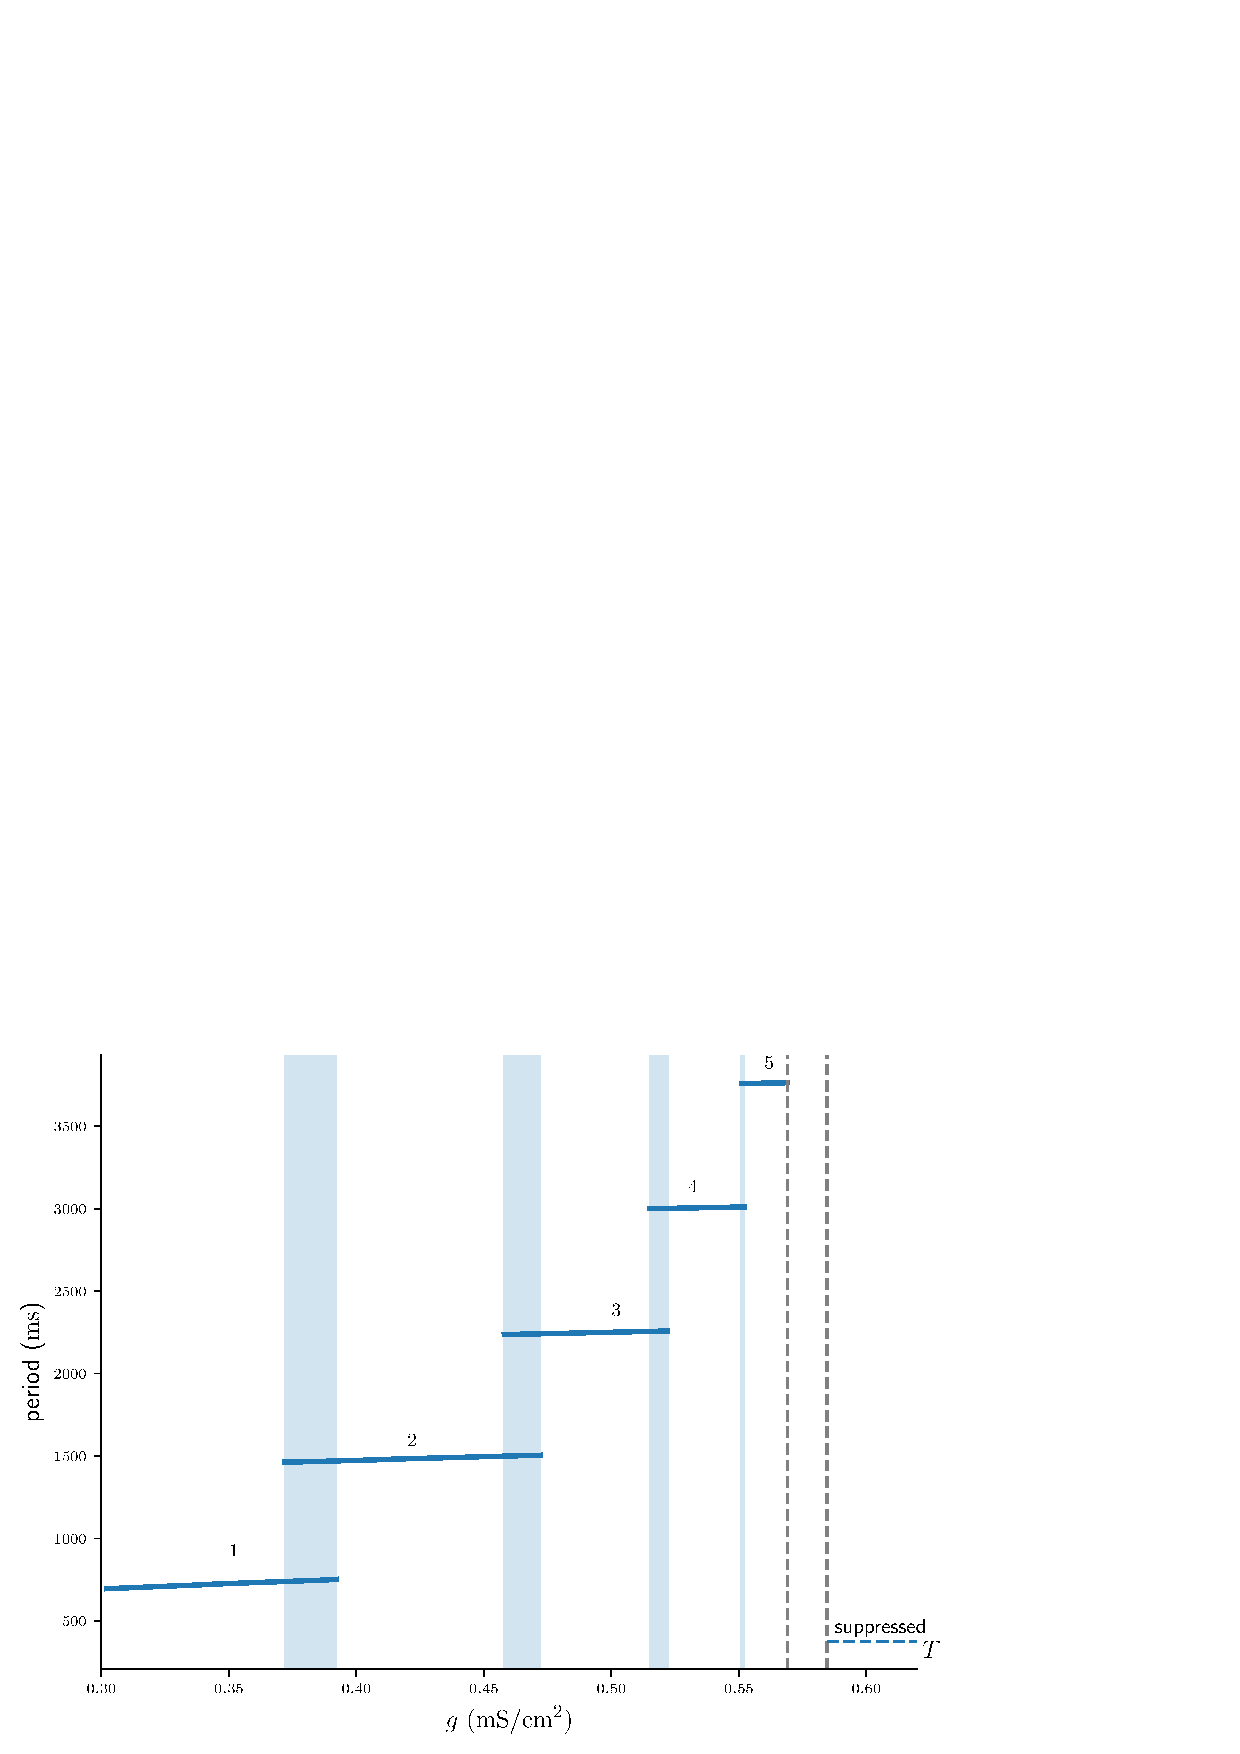
\includegraphics{fig/bif-diagram.pdf}
  \caption{Numerically computed bifurcation diagrams of stable $n-n$ solutions for increasing coupling strength $\gbar$. $\bm{\mathrm{(A)}}$ Period of stable solutions. Dashed lines show the interval between the $5-5$ and the suppressed solutions, where higher period $n-n$ solutions occur on increasingly smaller intervals of $\gbar$. $\bm{\mathrm{(B)}}$ $ISI$s corresponding to $n-n$ solutions in $\mathrm{(A)}$. Long $ISI$s are associated with the quiet phase of a burst, short $ISI$s with the free phase. During the free phase, $ISI$s are of approximately constant duration $T$.\label{fig:bif-diagram}}
\end{figure}

\begin{figure}[h!]
  \centering
  \includegraphics{fig/nullclines-coupled.pdf}
  \caption{Nullclines $v_{\infty}$ (blue) and $w_{\infty}$ (orange) in the $(v,w$)-phase plane for different values of the total synaptic conductance $\gbar s$. For small $\gbar s < g^{\star}$, fixed point $p_{f}$ is unstable (orange point). Larger values $\gbar s$ move $v_{\infty}$ down in the $(v,w)$-plane until $p_{f}$ changes stability (half orange,  half blue point) at some critical total conductance value $\gbar s = g^{\star}$, and becomes stable (blue point) for $\gbar>g^{\star}$.~\label{fig:nullclines-coupled}}
\end{figure}

\begin{figure}[h!]
  \centering
  \includegraphics[width=0.8\textwidth]{fig/release-delay.pdf}
  \caption{Numerically computed values of the release delay for varying $\gbar$. Each of the three branches (A, B, C) also shows the timecourse of the total synaptic conductance $\gbar s$ of a sample stable solution of both cells (blue and orange), as well as the release conductance $g^{\star}$ (dashed green line). $\bm{\mathrm{(A)}}$ Branch corresponding to the $1-1$ solution. Here the quiet cell only spikes after a significant release delay. $\bm{\mathrm{(B)}}$ Branch with a long release delay associated with a subset of $2-2$ solutions. Here the release condition is briefly satisfied after the first spike of cell 1. This does not cause firing of cell 2, which only occurs after the second spike of cell 1. $\bm{\mathrm{(C)}}$ Branch with $n-n$ solutions  where release delay is approximately zero and the release condition is sufficient for firing of cell 2.
   ~\label{fig:release-delay}}
\end{figure}

\begin{figure}[h!]
  \centering
  \includegraphics{fig/free-quiet.pdf}
  \caption{Schematic diagram of the free and quiet phases for a $3-3$ solution. $\bm{\mathrm{(A)}}$ Membrane potentials of cell 1 ($v_{1}$) and cell 2 ($v_{2}$).  The grey patches depict inter-burst-intervals $\delt$. $\bm{\mathrm{(B)}}$ Total synaptic conductance of cell 1 ($\gbar s_1$) as it crosses the release conductance $g^{\star}$. $\bm{\mathrm{(C)}}$ Solution $d_1(t)$ of depression variable of cell 1, during free (blue) and quiet phases (orange).~\label{fig:free-quiet1}}
\end{figure}

\begin{figure}[h!]
  \centering
  \includegraphics{fig/delta-t.pdf}
  \caption{Numerically computed bifurcation diagram of $\delt$ for varying $\gbar$. Each continuous branch is associated with a stable $n-n$ burst solution. Increasing $\gbar$ increases $\Delta t$ until the solutions bifurcate at $\Delta t\approx T$.~\label{fig:delta-t}}
\end{figure}

\begin{figure}[h!]
  \centering
  \includegraphics{fig/FQ-map.pdf}
  \caption{Maps $F_n$ $\bm{\mathrm{(A)}}$ and $Q_n$ $\bm{\mathrm{(B)}}$ for $\gbar=0.6$ $\si{mS/cm^{2}}$ and $n=1,2,3,4$. Curves $F_n$ intersect at $d_{s}$ which is indicated by a dashed vertical line.~\label{fig:FQ-map}}
\end{figure}

\begin{figure}[h!]
  \centering
  \includegraphics{fig/Pn-map.pdf}
  \caption{Map $\Pi_{n}:d^{\star}$. $\bm{\mathrm{(A)}}$ $\Pi_{n}$ for $n=1,2,3,4$ at $\gbar=0.6$ $\si{mS/cm^{2}}$. $\bm{\mathrm{(B)}}$ $\Pi_{2}$ with $n=2$ for varying $\gbar \approx 0.01, 0.034, 0.3$ $\si{mS/cm^{2}}$. The identity function is illustrated by a diagonal line.~\label{fig:Pn-map}}
\end{figure}

\begin{figure}[h!]
  \centering
  \includegraphics{fig/folds.pdf}
  \caption{$\bm{\mathrm{(A)}}$ Fold bifurcation diagrams of stable (continuous curves) and unstable (dotted curves) fixed points of $\Pi_{n}$ for varying $n$. $\bm{\mathrm{(B)}}$ Cycle periods computed from stable fixed points (blue), and the corresponding solution period from numerical integration of the system of ODEs (orange).~\label{fig:folds}}
\end{figure}

\begin{figure}[h!]
  \centering
  \includegraphics[width=0.8\textwidth]{fig/final-bif.pdf}
  \caption{Bifurcation diagrams of stable $n-n$ solutions computed analytically from fixed points of $\Pi_n$ and plotted on the respective intervals of $\gbar\in \big[\gbar_+(n),\gbar_-(n)\big]$ (blue), and computed from numerical integrations of the ODEs (orange).~\label{fig:final-bif}}
\end{figure}

\end{document}
